\documentclass[a4paper,11pt]{article}

\usepackage[width=165mm,top=30mm,bottom=35mm,bindingoffset=0mm]{geometry}
\usepackage{csquotes}
\usepackage{graphicx}
\graphicspath{{Pics/}}
\usepackage{float}
\usepackage{multirow}
\usepackage{subcaption}
\usepackage{siunitx}
\usepackage{amsmath,amssymb}
\usepackage{mathtools}
\usepackage{amsfonts}
\let\vec\mathbf

\usepackage{soul, color}

\usepackage[unicode=true]{hyperref}
\usepackage[table]{xcolor}
\hypersetup{
	colorlinks,
	linkcolor={red!40!black},
	%    citecolor={blue!50!black},
	urlcolor={blue!40!black}}

\usepackage{xcolor}
\definecolor{codegreen}{rgb}{0,0.6,0}
\definecolor{codegray}{rgb}{0.5,0.5,0.5}
\definecolor{codepurple}{rgb}{0.58,0,0.82}
\definecolor{backcolour}{rgb}{0.98,0.98,0.96}

\definecolor{ashgrey}{rgb}{0.6, 0.75, 0.71}
\definecolor{limegreen}{rgb}{0.2, 0.8, 0.2}
\definecolor{green(colorwheel)(x11green)}{rgb}{0.0, 1.0, 0.0}
\definecolor{dandelion}{rgb}{0.94, 0.88, 0.19}
\definecolor{pear}{rgb}{0.82, 0.89, 0.19}

\usepackage{listings}
\lstdefinestyle{mystyle}{
	backgroundcolor=\color{backcolour},
	commentstyle=\color{codegreen},
	keywordstyle=\color{magenta},
	numberstyle=\tiny\color{codegray},
	stringstyle=\color{codepurple},
	basicstyle=\ttfamily\footnotesize,
	breakatwhitespace=false,
	breaklines=true,
	captionpos=b,
	keepspaces=true,
	numbers=left,
	numbersep=5pt,
	showspaces=false,
	showstringspaces=false,
	showtabs=false,
	tabsize=2
}
\lstset{style=mystyle}

\setlength{\parindent}{0pt}
\setlength{\parskip}{1em}

\usepackage{booktabs}

%\renewcommand{\thesubsubsection}{\thesubsection.\alph{subsubsection}}
\renewcommand{\thesubsection}{\alph{subsection}}
\counterwithin*{subsection}{section}

\captionsetup[figure]{font=footnotesize,labelfont=normalsize}

\begin{document}

    \begin{titlepage}
\begin{center}
    \textbf{\LARGE Technion - Israel Institute of Technology}

    \vspace{1.5cm}

    
\includegraphics[width=0.4\linewidth]{logo}

    \vspace{2.5cm}

    \textbf{\LARGE Introduction to Artificial Intelligence}

    \vspace{1cm}

    {\Large Professor Oren Salzman}

    \vspace{2mm}

    {\Large TA Tal Swisa}

%    \vspace{3cm}
    \vfill

    \textbf{\Huge Homework 3}

    \vspace{2cm}

    \begin{tabular}[c]{ r l } % try with "r l" instead of "l l"
        Pietro BRACH DEL PREVER & 921210282\\
        Yaacov VAKSMAN  & 316153261\\

    \end{tabular}

    \vspace{2cm}

    {\normalsize January 27, 2021}

    \vspace{1mm}

    {\normalsize Academic Year 2021/2022}
\end{center}
\end{titlepage}


	\part*{Part B}
    \section*{Question 1}
    The statement is true. Let some node n in the ID3 Algorithm. Without the MinMax normalization, we choose to split by some continues feature $f$. After performing dynamic discretization we get that the highest information-gain value we can get is by using feature $f$ and some threshold value $t_{j}$ .

Let us now consider the MinMax normalization. let $x$ be the value of the feature, the normalized value is $x_{n}$ :
\begin{equation*}
    x_{n}=\frac{x-x_{min}}{x_{max}-x_{min}}=\frac{x}{x_{max}-x_{min}}-\frac{x_{min}}{x_{max}-x_{min}}
\end{equation*}

The normalization value is a linear function of the original value, and this is a monotonically increasing function. Thus, performing the dynamic discretization and the splitting by every feature will lead to the same results achieved without the normalization (the values by themselves are not important, the important thing is the order: if $x_{2}>x_{1}$ then $x_{n_{2}}>x_{n_{1}}$, so if the order of the examples haven't changed then the information gain won't change and we will chose the same feature and relative place to divide the examples by that feature, and thus the same tree will be built and the accuracy will be the same.

    \section*{Question 2}
    We define a possible heuristic for Nine Men's Morris as a weighted sum\footnote{The motivation of using that heuristic is from the paper: Simona-Alexandra PETCU, Stefan HOLBAN, \textit{Nine Men's Morris: Evaluation Functions}} based on the following rule:
\begin{equation*}
    h(s) = Evaluation(player)-Evaluation(rival) = \sum_i^N c_i\times R_i
\end{equation*}
If $h(s)>0$ white is supposed to be in a better condition, else black is.

The heuristic function we define is based on 8 contributions ($N=8$):
\begin{itemize}
    \item R1: returns 1 if a mill was closed by our player in he last move, returns -1 if a mill was closed by the opponent n the last move, returns 0 otherwise;
    \item R2: returns the difference between the number of my player's mills and the number of the rival's ones;
    \item R3: returns the difference between the number of my players' blocked pieces and the number of the rival's ones;
    \item R4: returns the difference between the number of my player's pieces and the number of the rival's ones;
    \item R5: returns the difference between the number of my player's 2-piece configurations and the number of the rival's ones (a 2-piece configuration is made by two soldiers and a free cell in a row), not accounting for the number of 2-piece configurations that compose the 3-piece configurations;
    \item R6: returns the difference between the number of my player's 3-piece configurations and the number of the rival's ones (a 3-piece configuration is made by two 2-piece configuration that shares a soldier);
    \item R7: returns the difference between the number of my player's double mills and the number of the rival's ones (a double mill is made by two mills that share a soldier);
    \item R8: returns 1 if a mill was closed by our player in he last move, returns -1 if a mill was closed by the opponent n the last move, returns 0 otherwise.
\end{itemize}
Different coefficients can be set for the different phases of the game.
    \section*{Question 3}
    \setcounter{subsection}{0}
    \subsubsection{}
The advantage of alpha-beta pruning algorithm is that it decreases the number of sub-trees explored and leaves evaluated, although the selected move will be the same selected by the minimax algorithm. Therefore, the optimality of the algorithm is maintained, but the runtime is decreased. By pruning branches, and eliminating all the computational cost of their expansion and leaves evaluation, a deeper search can be performed. This advantage is achieved by avoiding searching sub-trees of moves that will not be selected according to the current knowledge of the search tree.

Fig. \ref{fig:3_a_1} shows a scheme of how the alpha-beta pruning algorithm works.
\begin{figure}[h]
    \centering
    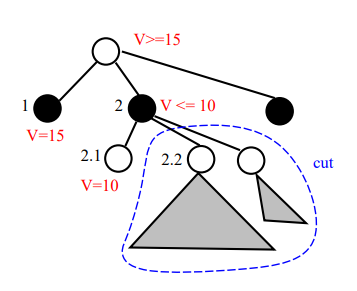
\includegraphics[width=0.5\linewidth]{3_a_1}
    \caption{Explanation of the alpha-beta pruning algorithm (cut-off version).}
    \label{fig:3_a_1}
\end{figure}
The algorithm explanation\footnote{Based on: Hsu TSAN-SHENG, \textit{Alpha-Beta Pruning: Algorithm and Analysis}}, in the cut-off version, follows (it references to Fig. \ref{fig:3_a_1}):
\begin{itemize}
    \item you explore branch at 1 and obtain the best value from it and call it $bound$ (10 in the case of the figure);
    \item You now search the branch at 2 by first searching the branch at 2.1;
    \item branch at 2.1 returns a value that is $\le bound$;
    \item in such a case there is no need to evaluate the branch at 2.2 and all later branches of 2, if any, at all since the best possible value for the branch at 2 must be $\le bound$;
    \item branch 2 cannot return a value better than the one returned from the branch at 1.
\end{itemize}

\subsubsection{}
Optimal pruning happens when the extreme (min or max) value of every node is found first: in nodes where we need to maximize the result, the highest minimax value should be found in the first child; in the nodes where we need to minimize the result, the lowest minimax value should be found in the first child, too.

\subsubsection{}
Fig. \ref{fig:3_0} shows how the algorithm works in practice on the example provided in the handout. No sub-tree or leave is pruned by the algorithm in this case.
\begin{figure}[h]
    \centering
    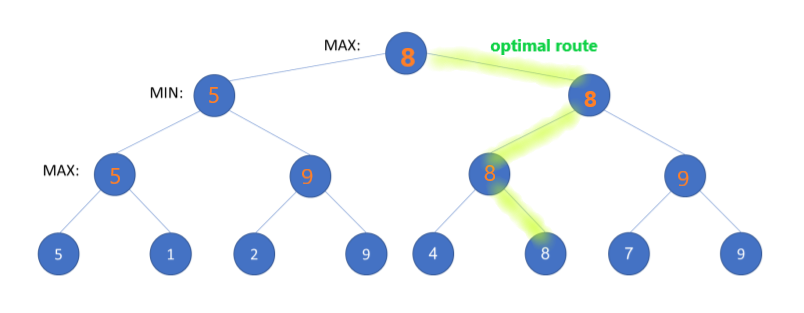
\includegraphics[width=0.6\linewidth]{3_0}
    \caption{Example of pruning according to the alpha-beta pruning algorithm.}
    \label{fig:3_0}
\end{figure}

	\part*{Part C}
%    \section*{Question 4}
%    The alpha-beta algorithm is based on the minimax algorithm: it returns the same result, but in a shorter time thanks to the pruning of some sub-trees. Minimax is an algorithm (often implemented in a recursive form as an iterative-deepening DFS) which is used to choose an optimal move for a player assuming that the other player is also playing optimally. Minimax strategy is safe, since it discourages taking any risks. Minimax generates the whole game tree, down to the leaves. Alpha beta pruning has no effect on the evaluation of the terminal states and returns the same result of minimax, i.e. the optimal result.

However, exploring the whole search tree is impossible in most cases, because it is too large and it would require too much resources, both in terms of time and of memory. What is performed instead is a search until a certain depth $d$ (often by means of an iterative-deepening DFS algorithm, as in our case) and the evaluation of the leaves of such trees (the last states reached and not expanded in the search). The evaluations is based on some heuristic functions. If we had a perfect heuristic we would need to perform the search and then the evaluation only one move ahead, but in reality the evaluation functions are always imperfect. The quality of the minimax algorithm, and therefore of the alpha-beta pruning algorithm, depends on its heuristic.  The statement is therefore false: the alpha-beta algorithm i would be optimal only with  a perfect heuristic, and this is not the case. To sum up, the terminal utilities of the final states are replaced by the evaluation function for non-terminal positions. Performing this change in the algorithm makes it non-optimal (but feasible).

Fig. \ref{fig:4} shows an example of a search-space where alpha-beta algorithm evaluates states at $depth=1$ and returns the optimal decision $a1$ according the evaluation (50 is the maximum value among the values computed for the child states), while the algorithm run until the terminal states (no heuristic, no evaluation, just the utility of the terminal states) of the search tree ($depth = 2$) would have returned $a3$: considering an optimal rival, $a1$ eventually returns $utility = 40$, while $a3$ returns a terminal state utility of 42.

\begin{figure}[h]
    \centering
    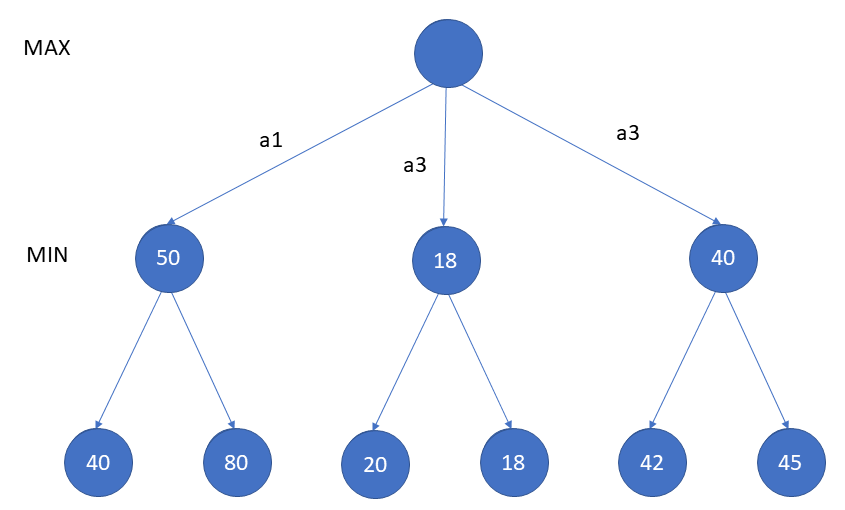
\includegraphics[width=0.6\linewidth]{4}
    \caption{Example of alpha-beta algorithm with heuristic and evaluation at $depth = 1$.}
    \label{fig:4}
\end{figure}
    \section*{Question 5}
    Let us suppose the finite states $s1,s2,s3,s4$. In zero-sum games $U(s,1)=-U(s,2)$ or $\sum_{k}^{N}U(s,k)=0$ sum of the utilities of all the players is zero for all states. For simplicity, let $U(s)=[U(s,1),U(s,2)]$.


\subsubsection{}
For the sake of the reasoning, we will assume that player 2 is optimal and that the following values represent the final utilities of the four states for each player:
\begin{align*}
    U(s1)&=[1,1] \\
    U(s2)&=[5,-3] \\
    U(s3)&=[0,0] \\
    U(s4)&=[1,-1]
\end{align*}

The diagram in Fig. \ref{fig:5_a} shows the corresponding non-zero sum game.
\begin{figure}[h]
    \centering
    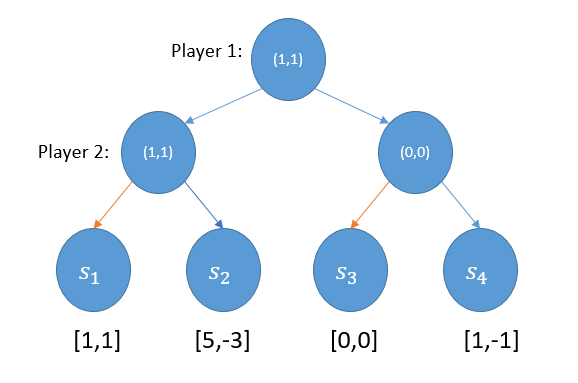
\includegraphics[width=0.6\linewidth]{5_a}
    \caption{Example of a non-zero sum game where the optimality of minimax holds.}
    \label{fig:5_a}
\end{figure}

In the example of Fig. \ref{fig:5_a}, minimax still returns the optimal value and the optimal move. Minimax is optimal because there is a negative correlation between the two players i.e. what is good for player 1 is bad for player 2. Player 1 can see that, for the opponent's optimal moves, the game can terminate either in state $[1,1]$ or in state $[0,0]$: indeed, player's 2 best moves are represented by the edges leaning to left in both cases (orange arrows). So minimizing player's 1 utility in the opponent move nodes was the same as maximize opponent utility. Hence, minimax is optimal in such an example.

\subsubsection{}
We now assume that the following values represent the final utilities of the four states for each player:
\begin{align*}
    U(s1)&=[1,1] \\
    U(s2)&=[-1,-1] \\
    U(s3)&=[2,0.5] \\
    U(s4)&=[-1.5,0]
\end{align*}

The diagram in Fig. \ref{fig:7_c_first} shows the corresponding non-zero sum game.
\begin{figure}[h]
    \centering
    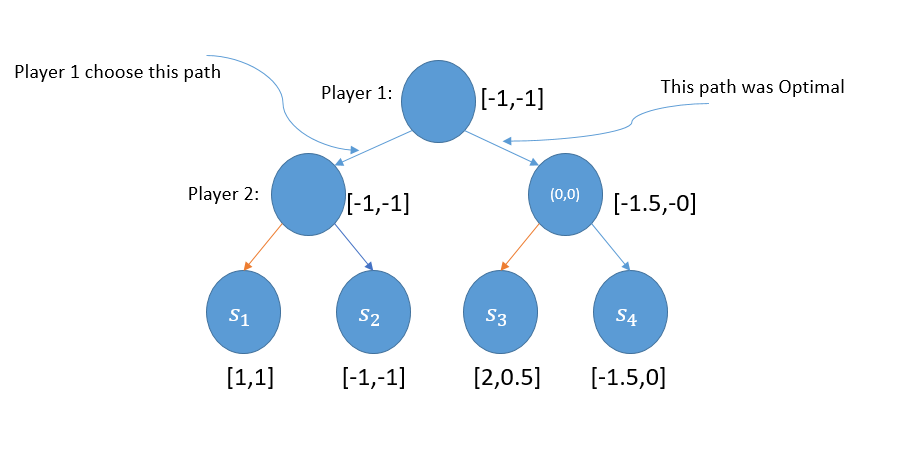
\includegraphics[width=0.8\linewidth]{7_c}
    \caption{Example of a non-zero sum game where the optimality of minimax does no hold.}
    \label{fig:7_c_first}
\end{figure}

The example in Fig. \ref{fig:7_c_first} shows a case where minimax is not optimal, i.e. does not perform the best moves. Minimax minimizes the utility of player 1 at the opponent nodes, but the optimal path instead would be given if it tried to maximize the opponents utility at the opponent's nodes.

Considering the specific example under the scope, the minimax algorithm would compute $[-1,-1]$ and $[-1.5,0]$ and would therefore chose to go left and get minimax value of $-1$, instead of $-1.5$. However, the opponent goes left in his nodes (orange arrows) during its turn, because that is how it can maximizes its terminal utility. Thus, considering this game-play, player 1 will get the terminal utility of 1. After a deeper analysis, the best move for player 1 was to go right, because then the opponent will take the lest node $[2,0.5]$ and player 1 terminal utility could be 2.

    \section*{Question 6}
    \setcounter{subsection}{0}
    A student implements an alpha-beta algorithm and in a game against the software she noticed that the computer didn't take a winning move (in the next step) and chose another move instead.

\subsubsection{}
Such a situation is possible because the heuristic can mislead the computer decisions and therefore avoid the wining move. In particular, the winning move has a lower heuristic value than the move eventually chosen. Probably, the used heuristic doesn't evaluate if the position represents a victory for the computer.

\subsubsection{}
The change that we can apply is quite simple: if the alpha-beta algorithm gets a state at $depth = 1$ that is winning for the computer, then it returns that move. In Lst. \ref{lst:ex6} we can see the regular alpha-beta algorithm pseudo-code with the slight modification required.% The changes proposed on the algorithm are listed in Table \ref{table:changes}.

\begin{lstlisting}[language=python, label={lst:ex6}, caption={Modified code: lines 2 to 4 have been added.}]
    alphaBeta(state):
        for successor in state.getSuccessors(): # added
            if successor.is_victory_for_player(): # added
                return successor # added
        return maxValue(state, -INFINITY, INFINITY, 0)

    maxValue(state, alpha, beta, depth):
        if cutoffTest(state, depth):
            return utility (state)
        value = -INFINITY
        for successor in state.getSuccessors():
            value= max(value, minValue(successor, alpha, beta, depth + 1))
            if value >= beta:
                return value
            alpha= max(alpha, value).
        return value

    minValue(state, alpha, beta, depth):
        if cutoffTest(state, depth):
            return utility(state)
        value = INFINITY
        for successor in state.getSuccessors():
        value=min(value, maxValue(successor, alpha, beta, depth + 1)
            if value <= alpha:
                return value
            beta min(beta, value)
        return value
\end{lstlisting}

%\begin{figure}[h]
%    \centering
%    \includegraphics[width=0.6\linewidth]{{6_b}}
%    \caption{Pseudo-code of the alpha-beta pruning algorithm.}
%    \label{fig:6b}
%\end{figure}
%
%\begin{table}[h]
%    \centering
%    \begin{tabular}{ r m{0.5\linewidth} }
%        \midrule
%        Portion of code & Explanation \\
%        \midrule
%        $G=G(state,agent)$ & So that it gets the agent, too. \\
%        \midrule
%        $G(state,agent)$ & it should return a tuple $(\{T,F\},\{T,F\})$. The first
%        boolean value is True if the state is endgame and the second is True
%        if it is victorious for the computer. \\
%        \midrule
%        $if G(state)\ is\ (True, True)$ & it should return return $-\infty$ or $\infty$ depending if the agent is respectively minimizing or maximizing the value. \\
%        \midrule
%        $if G(state)\ is\ (False, False)$ &  return $\pm\infty$ depending on the agent type, as above. \\
%        \midrule
%    \end{tabular}
%    \caption{Changes proposed to the algorithm.}
%    \label{table:changes}
%\end{table}
%
%\hl{TODO: check about the $\pm \infty$ value}

With such modifications we can guarantee that the winning move will always be returned.

	\part*{Part D}
    \section*{Question 7}
    Fig. \ref{fig:7_0} shows the search tree considered.
\begin{figure}[h]
    \centering
    \includegraphics[width=0.7\linewidth]{{7_0}}
    \caption{}
    \label{fig:7_0}
\end{figure}

\subsubsection{}
The expectimax of a chance node is calculated by a weighted sum of the utility and the probability to get it.
\begin{align*}
    U(B) &= 0.3\cdot5+0.7\cdot1=2.2 \\
    U(C) &= 0.4\cdot2+0.2\cdot3+0.4\cdot9=5 \\
    U(D) &= 0.1\cdot4+0.9\cdot7=6.7 \\
\end{align*}
The max operator takes the path with the best value at the chance node:
\begin{equation*}
    U(A)=U(argmax(U(i))=U(D)=6.7
\end{equation*}

\subsubsection{}
After this computation, it derives that action $D$ is the one we choose, therefore opting to explore the sub-tree through edge $a3$.

\subsubsection{}
It is not possible to trim in expectimax in the same way we prune sub-trees in alpha-beta algorithm. This is because it is not possible to calculate the expectimax value until all the nodes are evaluated. The pruning can be performed only if a higher and a lower bound of the leaves are available. The regular expectimax is calculated by means of Eq. \ref{eq:expectimax}, where $p,u$ are the probability and utility respectively.
\begin{equation}\label{eq:expectimax}
    Expectimax(state,action)=\sum_{i\in succ(state,action)}p_{i}u_{i}
\end{equation}

If we got an upper and lower bound of the utility $(u_{min},u_{max})$ we can predict the bounds of Expectimax node after revealing one possible successor:
\begin{equation*}
    Expectimax(state,action)\in[p_{1}\cdot u_{1}+(1-p_{1})\cdot u_{min},\ p_{1}\cdot u_{1}+(1-p_{1})\cdot u_{max}]
\end{equation*}
On the other had, if an upper and lower bound are not available, it is not possible to prune. An example is shown in Fig. \ref{fig:7_c}.
\begin{figure}[h]
    \centering
    \includegraphics[width=0.6\linewidth]{{7_c}}
    \caption{Example where pruning in expectimax compromises the correctness of the algorithm.}
    \label{fig:7_c}
\end{figure}
Assume the first action was been evaluated and the expectimin returned $5\times 0.3 + 1\times 0.7 = 2.2$. Now we need to evaluate the next action ($a2$). The first successor looks promising with high probability and value we already get 2.4 on our $a2$ chance node and it seems that we do not need to check the next leaves. However, what if the value in $D$ was negative and equals to $-2$? Than the result of the expectimin operator on the second action would be equal to $2$ (smaller then $a1$ action). That's why a naive approach will generally not work. Instead, if we had some bound on the leaves (e.g. positive value utility), we could say,as in the case of the above example, that after checking one leaf at the $a2$ action we could guarantee that action $a1$ is better.

    \section*{Question 8}
    \setcounter{subsection}{0}
    Lst. \ref{lst:ex8} shows the modification to the pseudo-code of alpha-beta to introduce a harder pruning, paying with returning the non-best results, worsened possibly by the factor $\epsilon$.

\begin{lstlisting}[language=python, label={lst:ex8}, caption={Modified code: the changes are in lines 110-11 and 21-22.}]
    alphaBeta(state):
        return maxValue(state, -INFINITY, INFINITY, 0)

    maxValue(state, alpha, beta, depth):
        if cutoffTest(state, depth):
            return utility (state)
        value = -INFINITY
        for successor in state.getSuccessors():
            value= max(value, minValue(successor, alpha, beta, depth + 1))
            if value + eps >= beta: # modified
                return value  + eps # modified
            alpha= max(alpha, value).
        return value

    minValue(state, alpha, beta, depth):
        if cutoffTest(state, depth):
            return utility(state)
        value = INFINITY
        for successor in state.getSuccessors():
            value=min(value, maxValue(successor, alpha, beta, depth + 1)
            if value - eps <= alpha: # modified
                return value - eps # modified
            beta min(beta, value)
        return value
\end{lstlisting}

The new algorithm returns a result different from the minimax in the case shown in Fig. \ref{fig:8_b}. In this case, alpha-beta prunes away the sub-tree after edge $a3$, and returns $a1$ with the optimal minimax value of 40. Minimax, on the other hand, returns $a3$ with optimal minimax value of 42.
\begin{figure}[h]
    \centering
    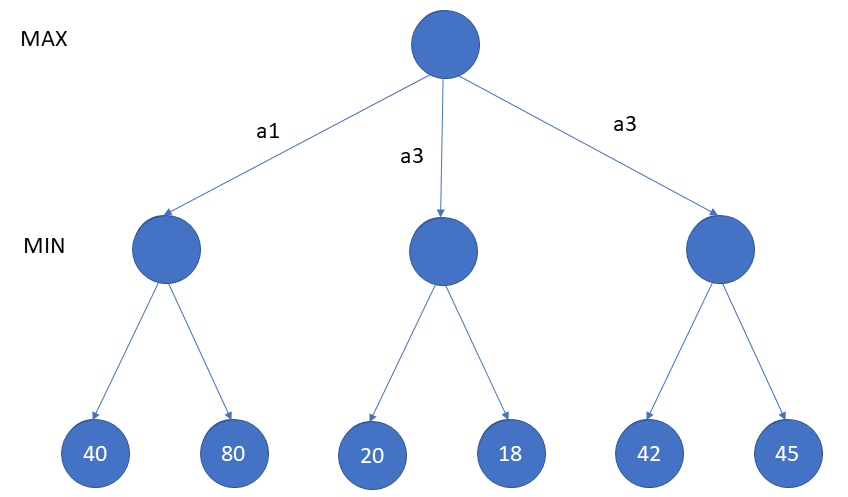
\includegraphics[width=1\linewidth]{8_b}
    \caption{With $\epsilon = 2.5$, $42 -\epsilon = 39.5 < 40$ and therefore alpha-beta modified prunes away the sub-tree child of edge $a3$.}
    \label{fig:8_b}
\end{figure}

%    \section*{Question 9}
%    \textbf{$\boldsymbol{d_{2}=\mathcal{O}(2\cdot d_{1}})$ }

\subsubsection{}
The time complexity of minimax is $O(b^{d})$, being function of the number ot leaves in the deepest searching layer. If we get the \lstinline!rival_move! we don't need to expand the whole opponent possible moves, but we just need to run this procedure and we already know among all the possible child nodes which one will be chosen by the rival through \lstinline!rival_move!. Thus the tree size multiply by $b$ every two layers of actions: the branching of the tree, i.e. the increase of the number of branches by a factor $b$, happen every two layer, and not one as before, since the opponent moves do not change the number of branches.
\begin{align*}
    O(b^{d_{1}}) &= O(b^{d_{2}/2}) \\
    d_{2} &= 2\cdot d_{1}
\end{align*}

\subsubsection{}
The minimax value is the highest value that the player can be sure to get without knowing the actions of the opponent, i.e it is the lowest value the rival can force the player to receive. Given state $s$, the ratio between the value of the minimax with use of the procedure and the value of the minimax without the use of the procedure when both runs are limited to depth $d$ is give by Eq. \ref{eq:minimax_ratio}.
\begin{equation}\label{eq:minimax_ratio}
    v_{i}=max(min(v_{i}))
\end{equation}
Indeed, minimax strategy assumes a optimal opponent, i.e. it assumes that the rival will chose its best scebario, which corresponds to our worst sceanrio, but the rival does not necessarily chooses the action with the lowest utility (the one with minimum minimax value). Thus, minimax value without using \lstinline!rival_move! procedure is always less or equal to the value of minimax with using \lstinline!rival_move! procedure.


\end{document}
